\documentclass[11pt,a4paper]{article}

\usepackage{amsmath,amssymb}
\usepackage{graphicx}
\usepackage{booktabs}
\usepackage{hyperref}
\usepackage[margin=2.5cm]{geometry}
\usepackage{caption}
\usepackage{subcaption}
\usepackage{placeins}
\usepackage{array}
\usepackage{url}
\hypersetup{hidelinks}
\emergencystretch=1em

\title{Two-Flash Multi-ROI Visual Detection Robustness\\for Mixed-Reality Multi-Agent HIL}
\date{\today}

\newcommand{\figdir}{figures}
\newcommand{\tabledir}{tables}

\begin{document}
\maketitle

\FloatBarrier

\section{Introduction}

The broader project investigates decentralised visual flashing as a mechanism
for coordinating multi-drone behaviour. Previous stages completed fixed-leader
visual HIL, a 1-virtual + 1-Pi mutual visual HIL comparison, and simulation
model selection in which EAPF Consensus was selected as the primary candidate
for the next 2-virtual + 1-Pi mixed-reality HIL stage. Before closing that
three-agent loop, the visual sensing layer must first demonstrate that the Pi
camera can observe two simultaneous virtual flashes as two independent event
streams.

This report therefore evaluates two-flash multi-ROI detection robustness. It
does not test synchronisation performance and does not alter the locked EAPF
Consensus parameters. It asks a narrower engineering question: can the Pi
automatically locate two browser-rendered flash targets, assign independent
ROIs to V0 and V1, detect each flash stream independently, and estimate
frequency accurately across visual conditions? The experiment is detection-only:
no EAPF closed-loop adaptation or Pi oscillator feedback is enabled. On the
available required evidence the detection pipeline is not yet fully ready for a
cautious 2V+1P EAPF smoke test under the full readiness gate. The corrected
contrast rerun supplies repeat-based evidence: medium contrast passed, whereas
low contrast failed because V0 produced no rising-edge detections.

\section{Experimental Objective}

The objective was to validate the visual detection layer for mixed-reality
multi-agent HIL. The readiness conditions covered baseline geometry,
moderately shifted positions, asymmetric and small target sizes, corrected
medium and low contrast settings, and several frequency relationships. Optional
stress conditions probed boundary cases and were not allowed to block the
readiness decision.

\section{Method}

\subsection{Detection-only setup}

The browser rendered two virtual flash targets, V0 and V1, at fixed screen
positions. The Pi camera observed both targets. For each condition the runner
first performed automatic simultaneous ROI calibration and then, where the
condition came from a formal batch, ran detection-only repeats. The Pi did not
run a closed-loop EAPF oscillator, did not flash a GPIO LED, and did not post
Pi flash events into a mutual synchronisation loop.

\subsection{Auto ROI calibration}

Auto ROI calibration used simultaneous two-target flashing. V0 and V1 were
configured with distinct frequencies when possible, typically 1\,Hz and
2\,Hz. The Pi captured a short frame sequence, computed a temporal-variation
image, found connected components, selected two non-overlapping candidate
regions, and assigned the components to V0 and V1 using the brightness-trace
frequency estimate. The resulting ROIs were then used by the multi-ROI detector.
Each ROI maintained independent signal history, adaptive normalisation,
hysteresis state, rising-edge detection, and duplicate suppression.

\subsection{Data selection}

\begin{table}[htbp]
\centering
\small
\begin{tabular}{p{0.20\textwidth}p{0.22\textwidth}p{0.12\textwidth}p{0.13\textwidth}p{0.23\textwidth}}
\toprule
Dataset & Purpose & Repeats & Duration & Notes \\
\midrule
\scriptsize\path{20260624_163557_formal_detection_batch} & Main formal detection batch & 3 & 30.0 & Used for baseline, position, size, frequency, and original stress conditions. Original contrast rows excluded from final contrast evidence. \\
\scriptsize\path{20260625_152611_contrast_rerun_corrected} & Corrected contrast repeat batch & 3 & 30.0 & Used for final medium- and low-contrast recall and frequency-error metrics. \\
\scriptsize\path{20260624_173430_contrast_visual_debug} & Previous contrast/display debug run & 0 detection repeats & approx. 6 s auto-ROI capture & Optional historical display evidence only; not used for final contrast recall or frequency metrics. \\
\scriptsize\path{20260624_175949_small_low_contrast_stress} & Small + low contrast stress batch & 3 & 30.0 & Optional stress condition; not part of readiness gate. \\
\bottomrule
\end{tabular}
\caption{Datasets used in this report.}
\label{tab:datasets}
\end{table}

The main formal batch is used for baseline, position, size, frequency, and
general stress results. The original contrast rows from that batch are not used
as final contrast evidence because the display pathway was later debugged.
Final medium- and low-contrast recall and frequency-error metrics are taken
from the corrected contrast repeat batch. The older contrast visual debug
folder is retained only as optional historical display evidence and is not used
for final contrast performance metrics.

\begin{table}[htbp]
\centering
\small
\begin{tabular}{p{0.25\textwidth}p{0.12\textwidth}p{0.12\textwidth}p{0.18\textwidth}p{0.23\textwidth}}
\toprule
Condition & Category & Required & Visual setting & Frequency setting \\
\midrule
Baseline & baseline & yes & high contrast & V0/V1 1/2 Hz \\
Shifted position & position & yes & high contrast & V0/V1 1/2 Hz \\
Large-small size & size & yes & high contrast & V0/V1 1/2 Hz \\
Small-small size & size & yes & high contrast & V0/V1 1/2 Hz \\
1.5/2.5 Hz & frequency & yes & high contrast & V0/V1 1.5/2.5 Hz \\
2 Hz phase offset & frequency & yes & high contrast & V0/V1 2/2 Hz \\
2 Hz near-simultaneous & frequency & yes & high contrast & V0/V1 2/2 Hz \\
Medium contrast & contrast & yes & bg 40, off 40, on 180 & V0/V1 1/2 Hz \\
Low contrast & contrast & yes & bg 80, off 80, on 120 & V0/V1 1/2 Hz \\
Too-close stress & position & no & high contrast & V0/V1 1/2 Hz \\
Tiny-small stress & size & no & high contrast & V0/V1 1/2 Hz \\
Small low-contrast stress & stress & no & bg 80, off 80, on 120 & V0/V1 1/2 Hz \\
\bottomrule
\end{tabular}
\caption{Step5c1 condition set and display settings.}
\label{tab:conditions}
\end{table}

\section{Results}

\subsection{Required-condition detection performance}

The repeat-based required conditions are shown together in
Figures~\ref{fig:recall} and~\ref{fig:freqerr}. Baseline, position, size,
and frequency rows come from the main formal batch; medium and low contrast
come from the corrected contrast repeat batch. 8 of 9
required conditions passed. The failed required condition was Low contrast.

\begin{table}[htbp]
\centering
\small
\begin{tabular}{p{0.26\textwidth}rrrrcc}
\toprule
Condition & V0 recall & V1 recall & V0 $|e_f|$ & V1 $|e_f|$ & Auto ROI & Pass \\
\midrule
Baseline & 0.989 & 0.989 & 0.0005 & 0.0010 & yes & yes \\
Shifted position & 0.989 & 0.983 & 0.0005 & 0.0010 & yes & yes \\
Large-small size & 0.978 & 0.983 & 0.0005 & 0.0010 & yes & yes \\
Small-small size & 0.989 & 0.989 & 0.0005 & 0.0010 & yes & yes \\
1.5/2.5 Hz & 0.978 & 0.987 & 0.0008 & 0.0013 & yes & yes \\
2 Hz phase offset & 0.989 & 0.983 & 0.0010 & 0.0010 & yes & yes \\
2 Hz near-simultaneous & 0.989 & 0.989 & 0.0010 & 0.0010 & yes & yes \\
Medium contrast & 0.933 & 0.983 & 0.0005 & 0.0010 & yes & yes \\
Low contrast & 0.000 & 0.983 & -- & 0.0013 & yes & no \\
\bottomrule
\end{tabular}
\caption{Repeat-based required-condition results. Medium and low contrast use the corrected contrast rerun.}
\label{tab:results}
\end{table}

\begin{figure}[htbp]
\centering

\includegraphics[width=0.95\textwidth]{\figdir/fig1_detection_recall_by_condition.pdf}
\caption{Detection count recall for required conditions. Baseline, position,
size, and frequency rows use the main formal batch; medium and low contrast use
the corrected contrast repeat batch.}
\label{fig:recall}
\end{figure}

\begin{figure}[htbp]
\centering

\includegraphics[width=0.95\textwidth]{\figdir/fig2_frequency_error_by_condition.pdf}
\caption{Detected frequency absolute error for repeat-based required
conditions. The y-axis is scaled to show the observed errors; the 0.10\,Hz pass
threshold is far above this plotted range.}
\label{fig:freqerr}
\end{figure}
\FloatBarrier

\subsection{Corrected contrast repeat validation}

The frontend/server/browser contrast pathway was debugged after the original
formal batch. The corrected contrast repeat folder was inspected for
\texttt{batch\_summary.json}, \texttt{batch\_summary.csv}, condition
folders, repeat folders, per-repeat \texttt{metrics\_summary.json}, and
\texttt{pi\_detection\_roi.csv} logs. Corrected contrast repeat detection data are complete and usable. Medium
contrast passed the repeat-based threshold. Low contrast failed because V0 had
zero detected rising edges across the three repeats; V1 remained detectable.

\begin{table}[htbp]
\centering
\small
\begin{tabular}{p{0.24\textwidth}rrrrcc}
\toprule
Condition & V0 recall & V1 recall & V0 $|e_f|$ & V1 $|e_f|$ & Auto ROI & Pass \\
\midrule
Medium contrast & 0.933 & 0.983 & 0.0005 & 0.0010 & valid & yes \\
Low contrast & 0.000 & 0.983 & -- & 0.0013 & valid & no \\
\bottomrule
\end{tabular}
\caption{Corrected contrast repeat validation from the corrected rerun.}
\label{tab:contrast}
\end{table}

\begin{figure}[htbp]
\centering

\includegraphics[width=0.95\textwidth]{\figdir/fig3_contrast_validation.pdf}
\caption{Corrected contrast repeat validation. Count recall and ROI-local
signal range show that medium contrast remained detectable, while low contrast
suppressed V0 detection under the current camera/display setup.}
\label{fig:contrast_validation}
\end{figure}
\FloatBarrier

\subsection{Auto ROI and ROI-local signal evidence}

Auto ROI calibration was valid for all required conditions, including the
corrected contrast repeats. The required-condition failure in low contrast was
therefore not an ROI-localisation failure; it was a detection-threshold/signal
amplitude failure for V0 during the repeat trials. ROI-local signal range is
reported because it is more informative than a full-frame background mean when
the camera frame includes bright non-target regions.

\begin{figure}[htbp]
\centering

\includegraphics[width=0.95\textwidth]{\figdir/fig4_auto_roi_validity.pdf}
\caption{Auto ROI calibration validity across required and optional stress
conditions. The too-close stress case failed auto-ROI validation and was not
part of the readiness gate.}
\label{fig:auto_roi}
\end{figure}

\begin{figure}[htbp]
\centering

\includegraphics[width=0.95\textwidth]{\figdir/fig5_signal_range_by_condition.pdf}
\caption{ROI-local signal range by condition. ROI-local metrics are preferred
over global background contrast because camera frames can include bright
non-target regions such as browser chrome or window borders.}
\label{fig:signal_range}
\end{figure}

\begin{figure}[htbp]
\centering

\includegraphics[width=0.95\textwidth]{\figdir/fig6_baseline_auto_roi_example.png}
\caption{Representative successful baseline auto-ROI calibration: selected
ROIs, temporal variation image, and threshold mask.}
\label{fig:baseline_auto_roi}
\end{figure}

\begin{figure}[htbp]
\centering

\includegraphics[width=0.95\textwidth]{\figdir/fig7_low_contrast_camera_evidence.png}
\caption{Corrected low-contrast camera evidence from the contrast rerun. The
global frame background mean is not used as the primary contrast metric because
non-target regions can dominate it; ROI-local signal ranges and trace
frequencies provide the more relevant evidence.}
\label{fig:contrast_evidence}
\end{figure}
\FloatBarrier

\subsection{Optional stress conditions}

Optional stress conditions were analysed separately from the readiness gate.
They are intended to reveal visual boundary cases rather than to define the
geometry for the first 2V+1P smoke test. The too-close stress condition failed
before repeats because the calibration could not produce a valid two-ROI
configuration. The tiny-small stress condition passed and therefore provides
additional evidence of size robustness. The small low-contrast stress condition
failed on V0 detection while V1 remained detectable, marking a combined
small-target/low-contrast boundary case.

\begin{table}[htbp]
\centering
\small
\begin{tabular}{p{0.26\textwidth}p{0.17\textwidth}p{0.17\textwidth}p{0.30\textwidth}}
\toprule
Stress condition & Auto ROI & Detection result & Interpretation \\
\midrule
Too-close stress & invalid & auto-ROI failed; repeats skipped & Intentionally difficult; failure indicates a boundary case when large halos nearly touch or padded ROIs overlap. Not representative of the intended 2V+1P layout. \\
Tiny-small stress & valid & pass & Passed; this optional very-small-target condition shows additional size robustness. \\
Small low-contrast stress & valid & boundary/fail & Optional combined small-target low-contrast stress. Failure does not block readiness, but marks a difficult visual boundary case. \\
\bottomrule
\end{tabular}
\caption{Optional stress outcomes.}
\label{tab:stress}
\end{table}

\subsection{Readiness for 2V+1P EAPF smoke}

The readiness decision is based on required conditions only. 8 of
9 repeat-based required conditions passed. Medium contrast
passed, but low contrast failed on V0 detection. Under the current readiness
gate the detection system is therefore not yet fully ready for a formal 2V+1P
EAPF smoke test that must include the low-contrast setting. A cautious smoke
test remains technically defensible only if the display/camera setup uses the
validated high- or medium-contrast operating range.

\section{Discussion}

The main formal batch supports the core two-flash detection pipeline. All
required non-contrast conditions passed the count-recall and frequency-error
thresholds, with auto ROI calibration valid and overlap ratios at zero. The
moderately shifted position condition passed, indicating that the connected
component based auto-ROI procedure is not tied to only one screen placement.
The size conditions also passed, including the required small-small case.

The corrected contrast evidence changes the readiness interpretation. The
frontend/server/browser pathway can apply separate baseline, medium, and low
brightness settings, and auto ROI calibration remained valid. However, the
repeat detector failed for V0 in the low-contrast condition. This makes low
contrast a practical lower bound for the current detector/camera exposure
configuration rather than a passed robustness condition.

Optional stress conditions behaved as useful boundary probes. The
position-too-close stress condition was intentionally difficult: large flash
halos were nearly touching, so padded ROIs could become ambiguous. Its failure
does not represent the intended 2V+1P layout and does not block readiness. The
tiny-small and small-low-contrast stress conditions are likewise reported as
limits rather than required success criteria.

\subsection{Limitations}

First, low contrast failed for V0 under the current camera/display setup, so
the low-contrast setting should be avoided or retuned before formal closed-loop
testing. Second, camera auto-exposure and bright non-target regions can make a full-frame
background mean misleading; ROI-local signal range is the preferred contrast
metric here. Third, the experiments use browser-rendered targets rather than
two physical drone LEDs. Fourth, passing detection-only tests does not prove
closed-loop 2V+1P synchronisation stability; it only validates that the visual
event streams are sufficiently separable to attempt a smoke test.

\section{Conclusion}

The Step5c1 evidence supports the core two-flash detection pipeline in the
validated high- and medium-contrast operating range, but it does not pass the
full required robustness gate because low contrast failed for V0. The next
2V+1P EAPF smoke test should therefore either use the validated contrast range
or first improve/retune low-contrast detection. Stress condition failures
should be interpreted as boundary cases, not blockers for the intended
smoke-test geometry.

\appendix

\section{Validation Tables}

The merged machine-readable analysis table is saved as
\path{derived/merged_condition_summary.csv}, and per-repeat rows used from
formal detection batches are saved as
\path{derived/merged_repeat_rows.csv}.
The corrected contrast repeat-data inspection is saved as
\path{derived/contrast_repeat_inspection.json}.
Any missing appendix image panels or generation warnings are saved as
\path{derived/generation_warnings.json}.

\section{Diagnostic Images}

The following appendix grids copy representative diagnostics into this report
folder. They are curated from the raw logs; the raw experiment folders are not
modified.


\begin{figure}[htbp]
\centering
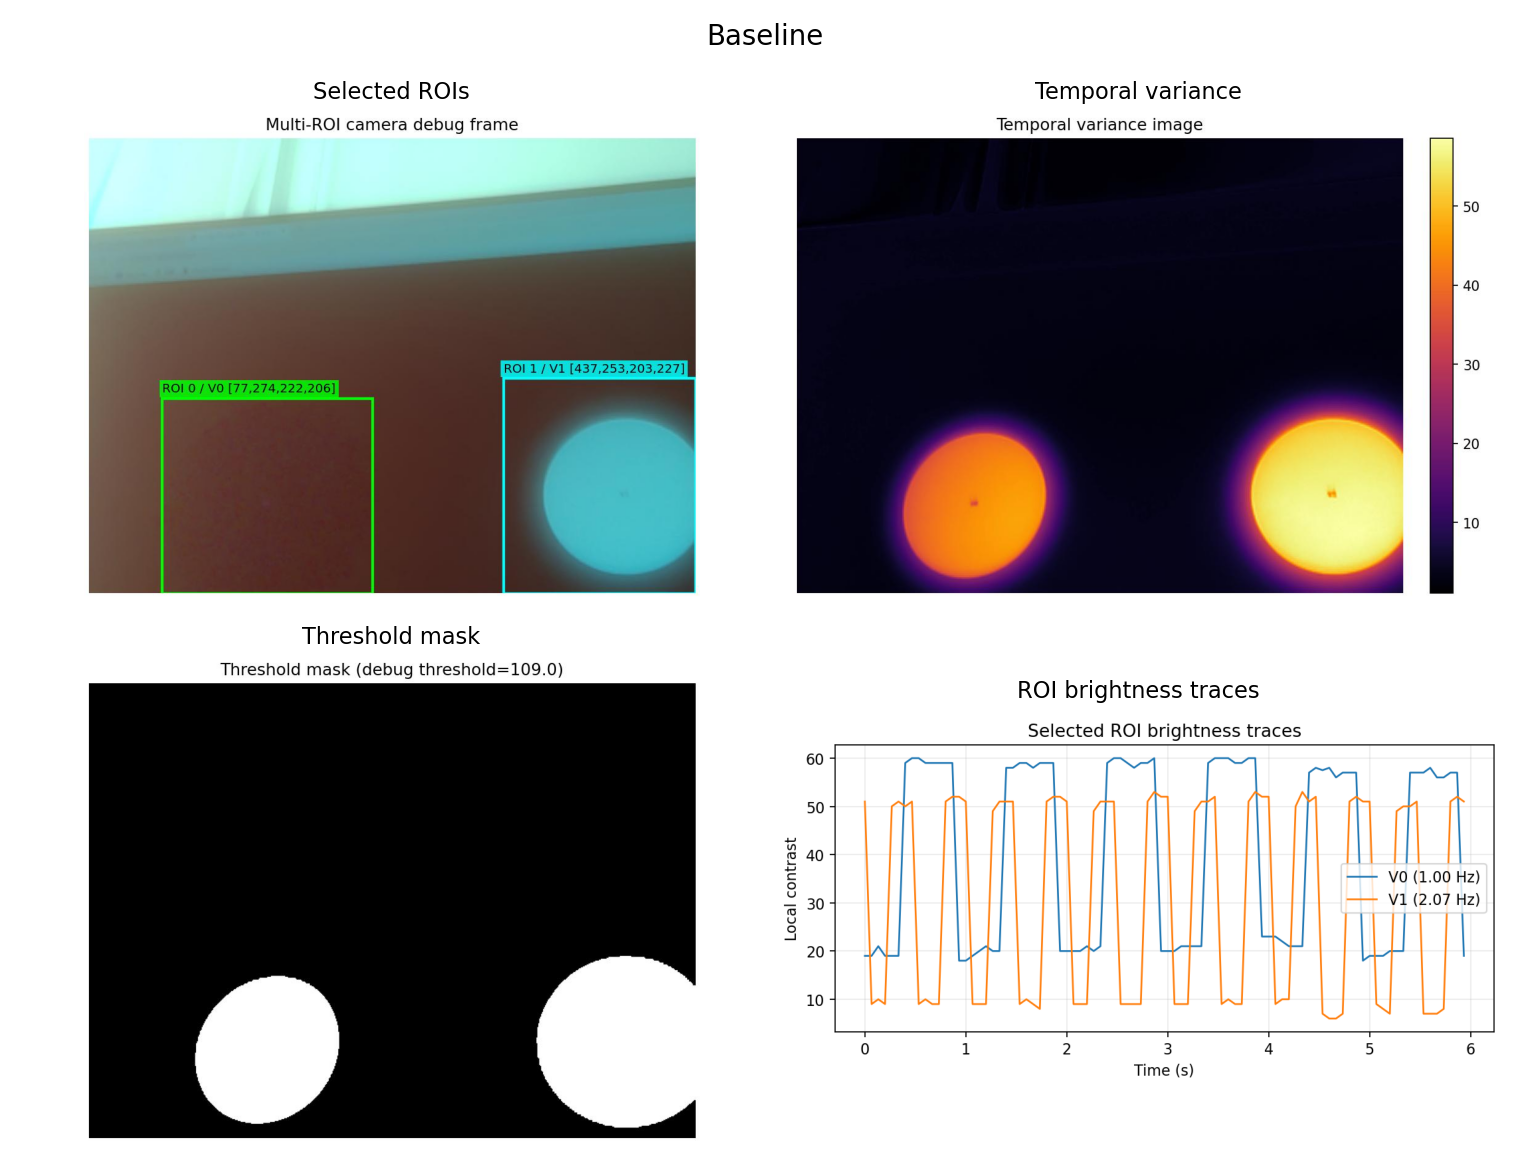
\includegraphics[width=0.95\textwidth]{figures/appendix/baseline_diagnostic_grid.png}
\caption{Auto-ROI diagnostics for Baseline.}
\end{figure}

\begin{figure}[htbp]
\centering
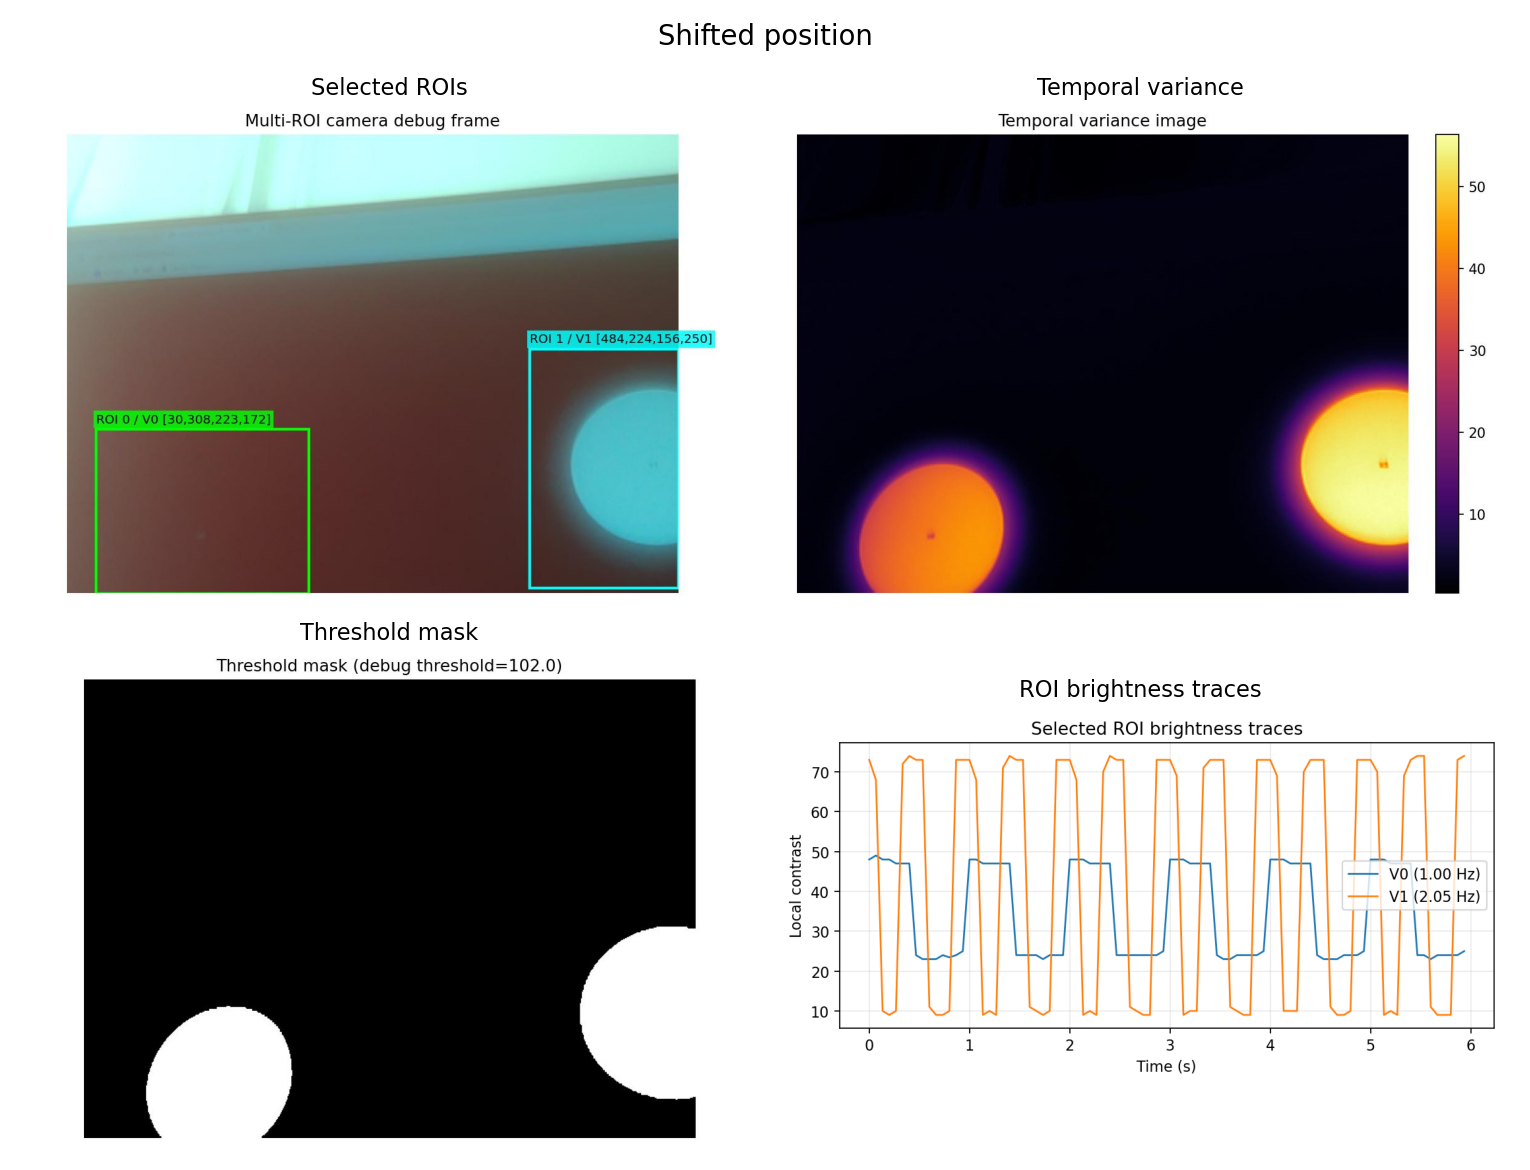
\includegraphics[width=0.95\textwidth]{figures/appendix/position_shifted_diagnostic_grid.png}
\caption{Auto-ROI diagnostics for Shifted position.}
\end{figure}

\begin{figure}[htbp]
\centering
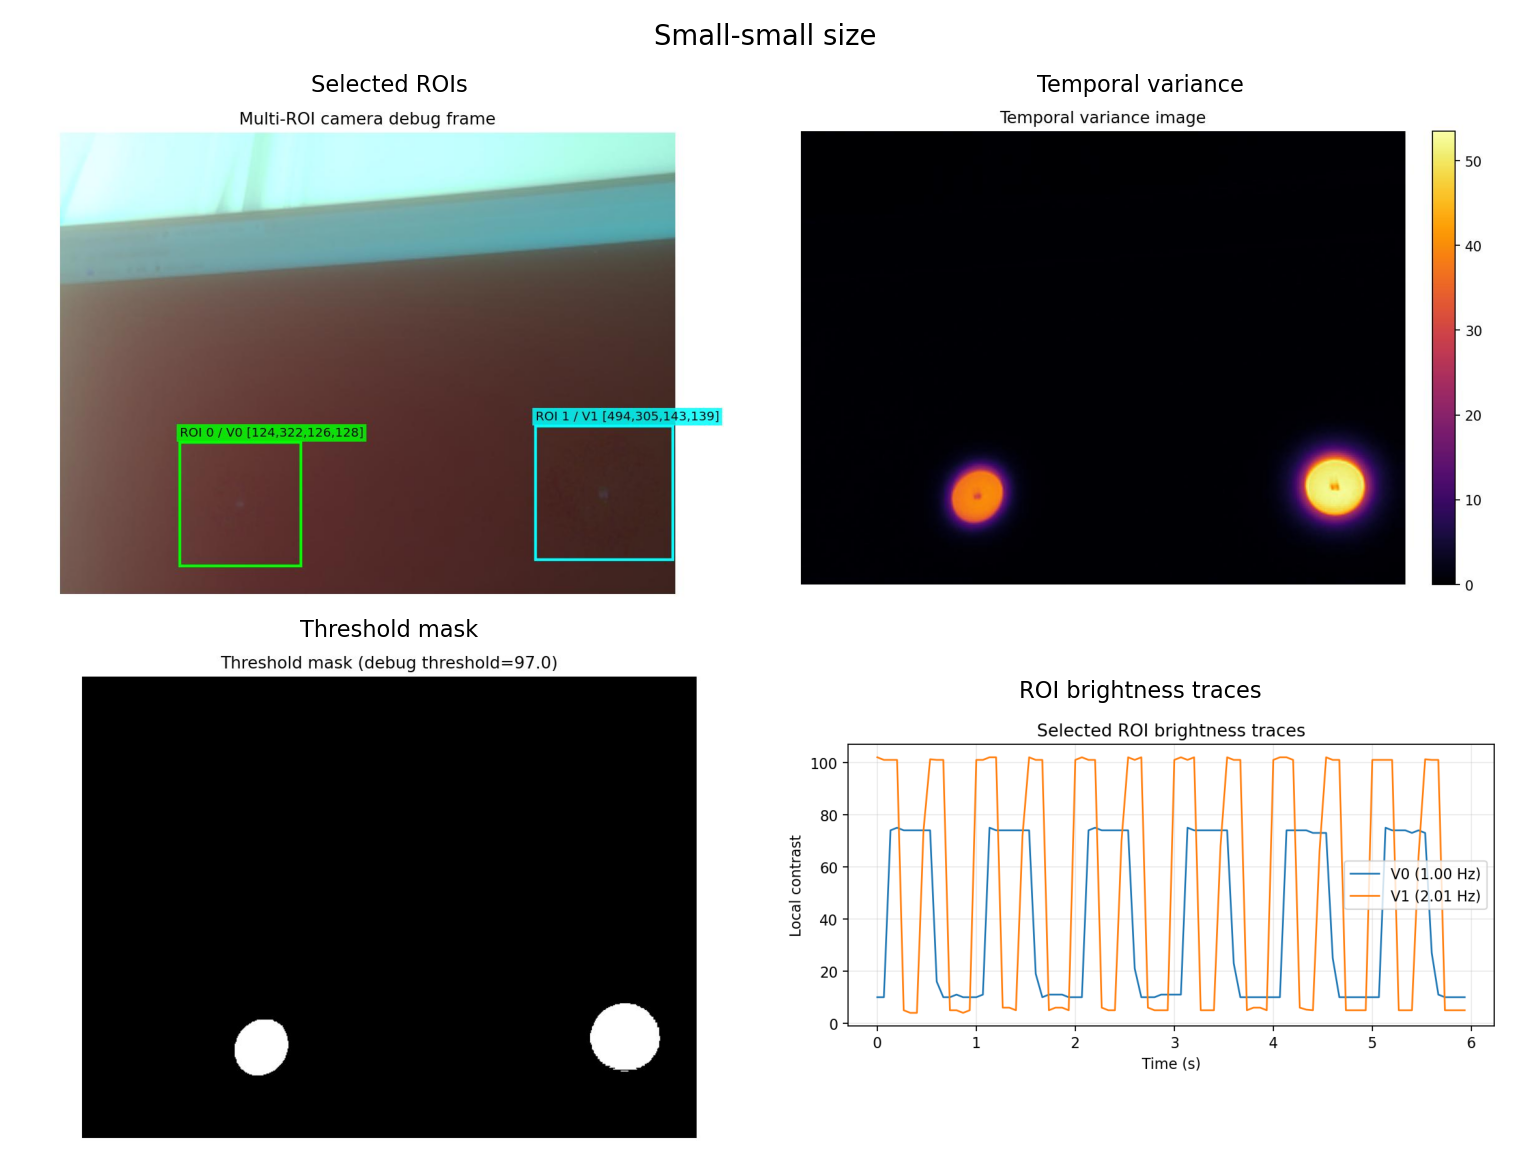
\includegraphics[width=0.95\textwidth]{figures/appendix/size_small_small_diagnostic_grid.png}
\caption{Auto-ROI diagnostics for Small-small size.}
\end{figure}

\begin{figure}[htbp]
\centering
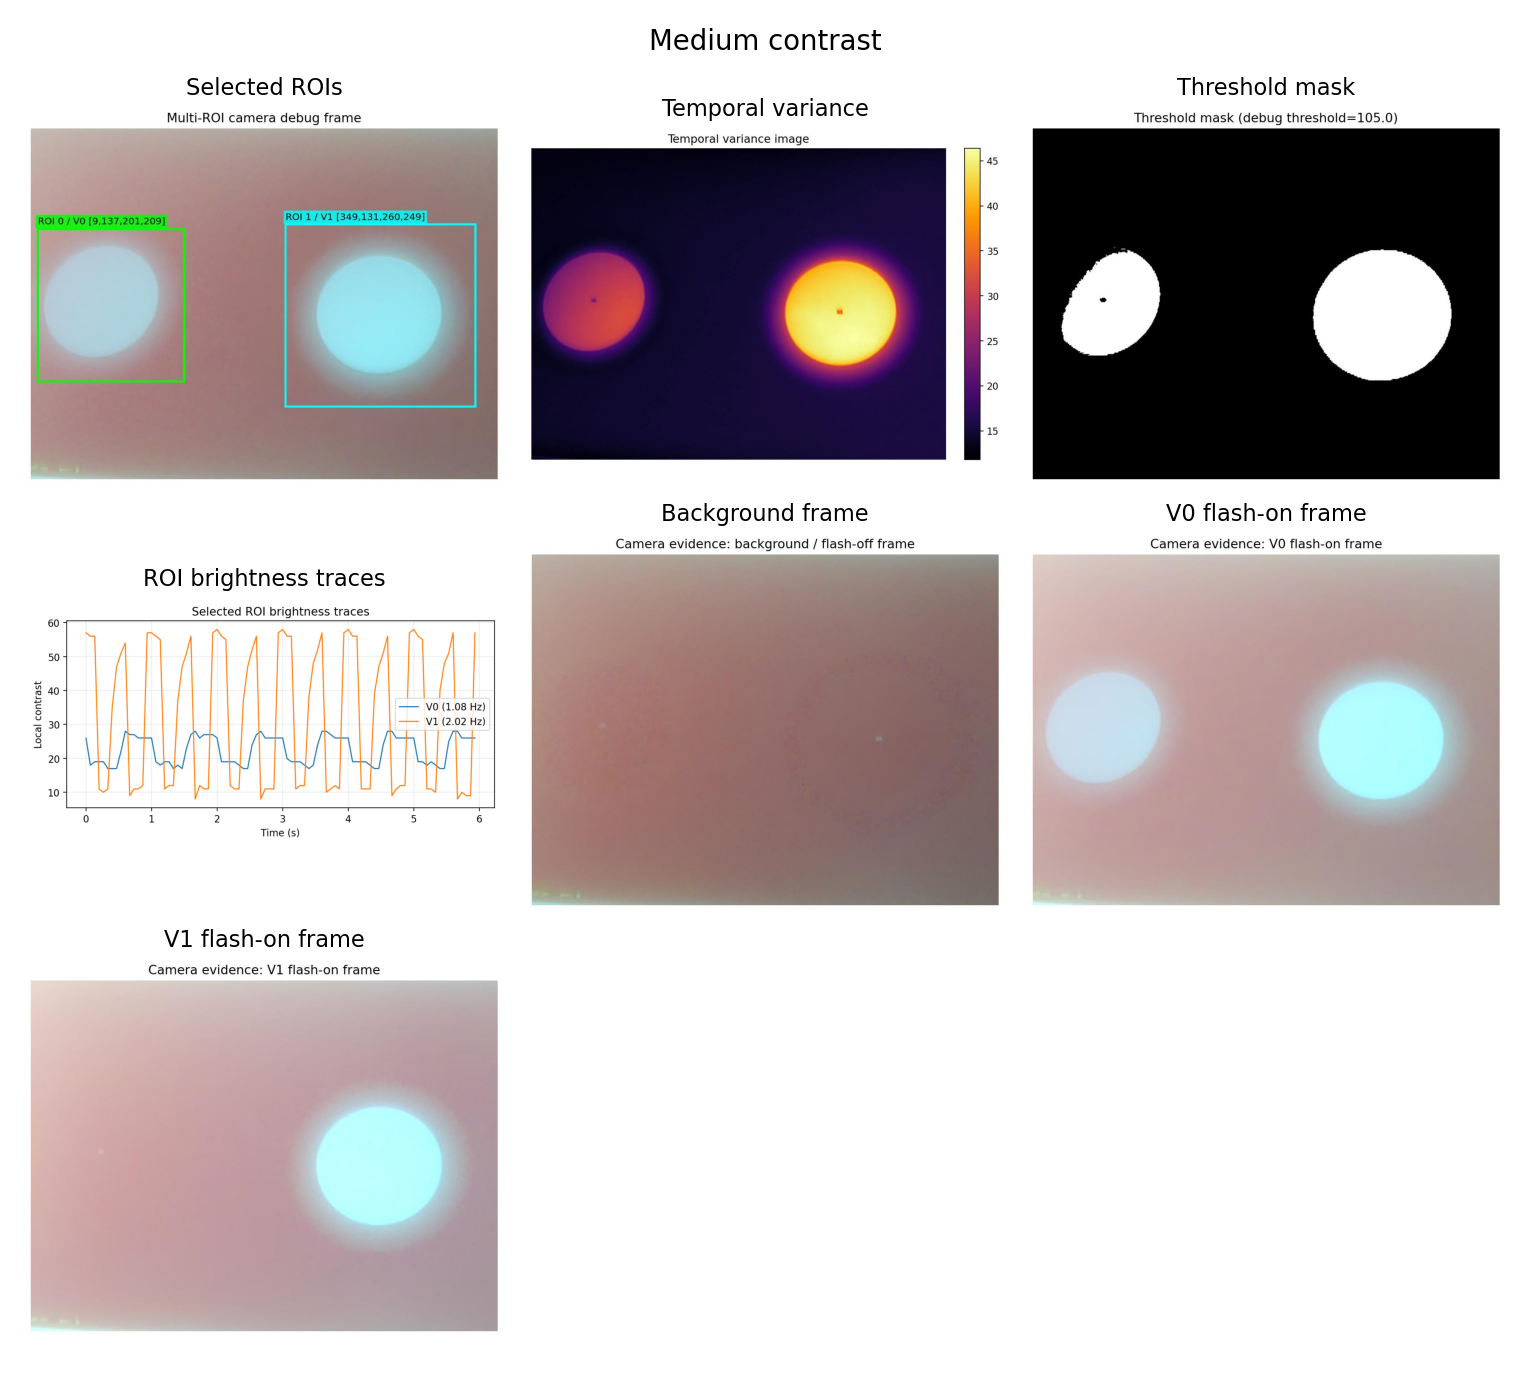
\includegraphics[width=0.95\textwidth]{figures/appendix/contrast_medium_diagnostic_grid.png}
\caption{Auto-ROI diagnostics for Medium contrast.}
\end{figure}

\begin{figure}[htbp]
\centering
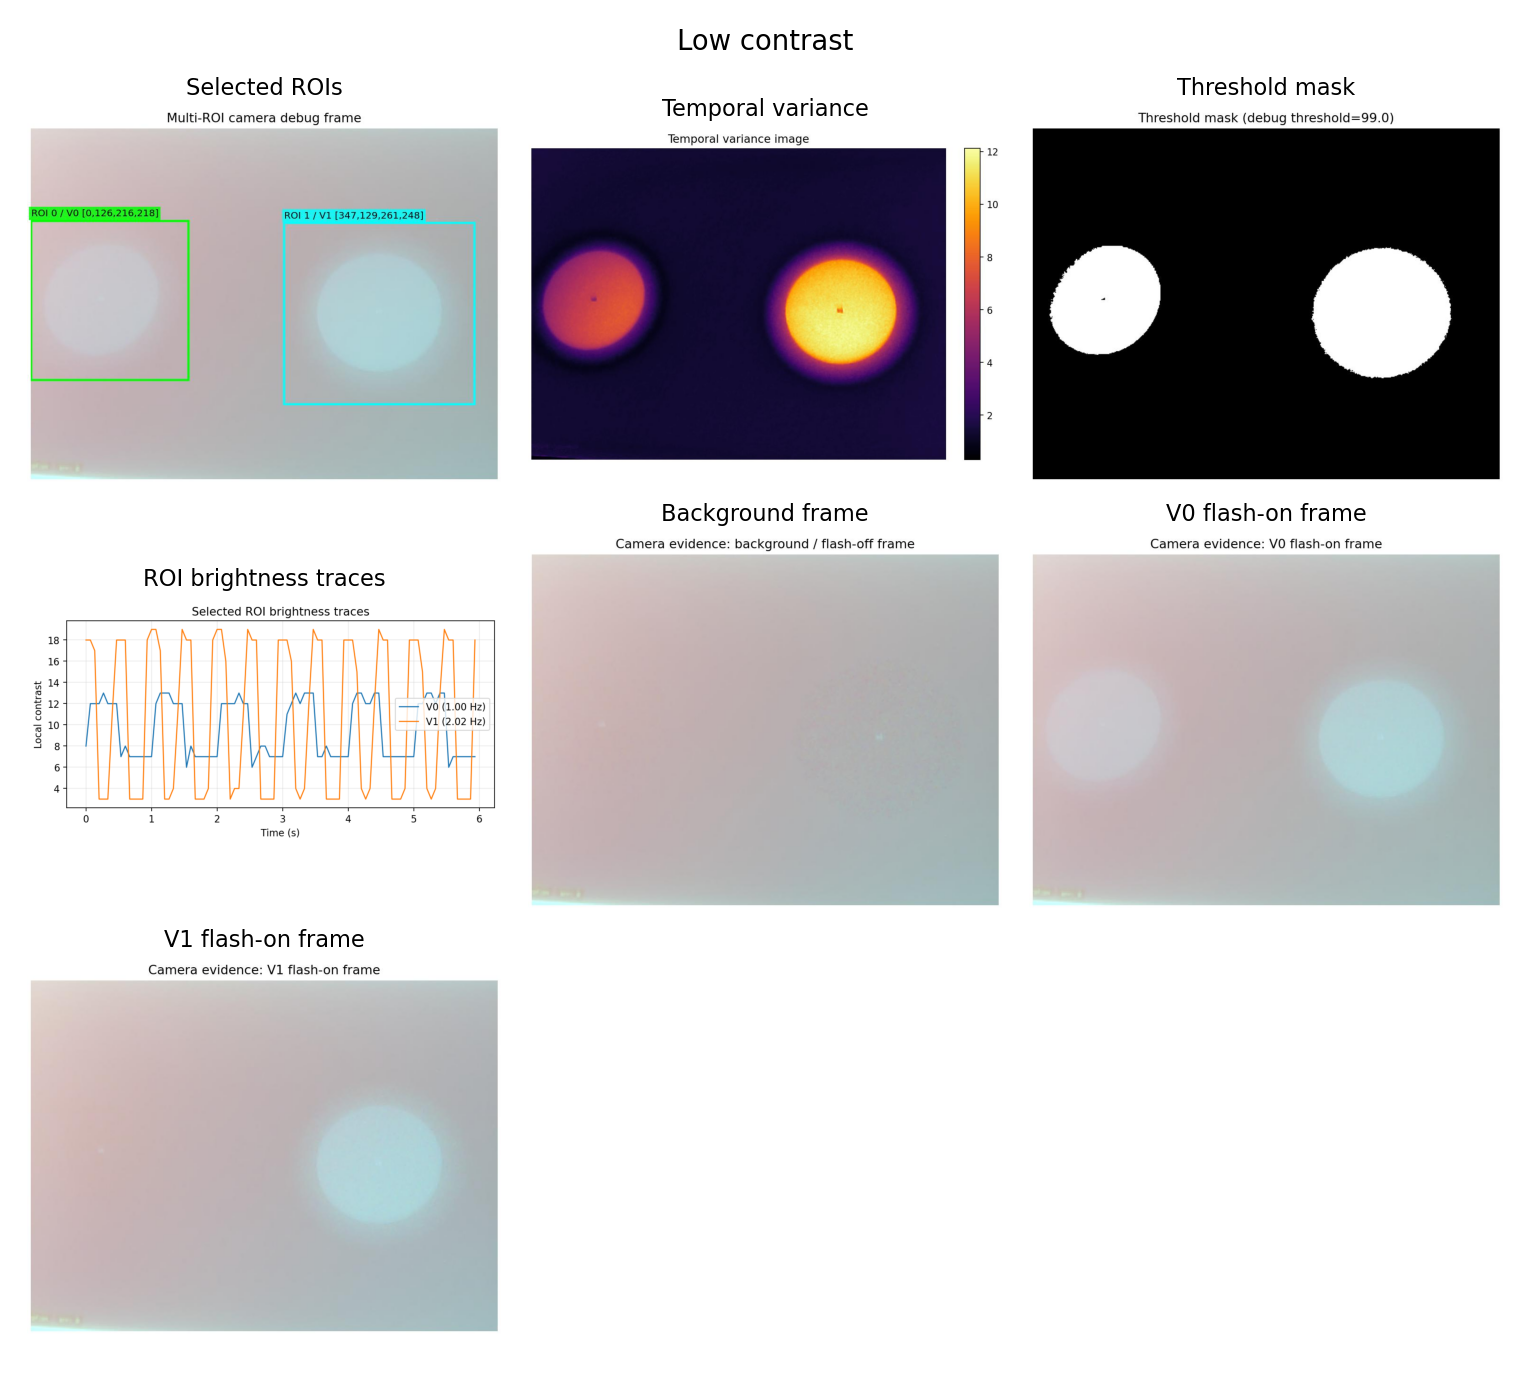
\includegraphics[width=0.95\textwidth]{figures/appendix/contrast_low_diagnostic_grid.png}
\caption{Auto-ROI diagnostics for Low contrast.}
\end{figure}

\begin{figure}[htbp]
\centering
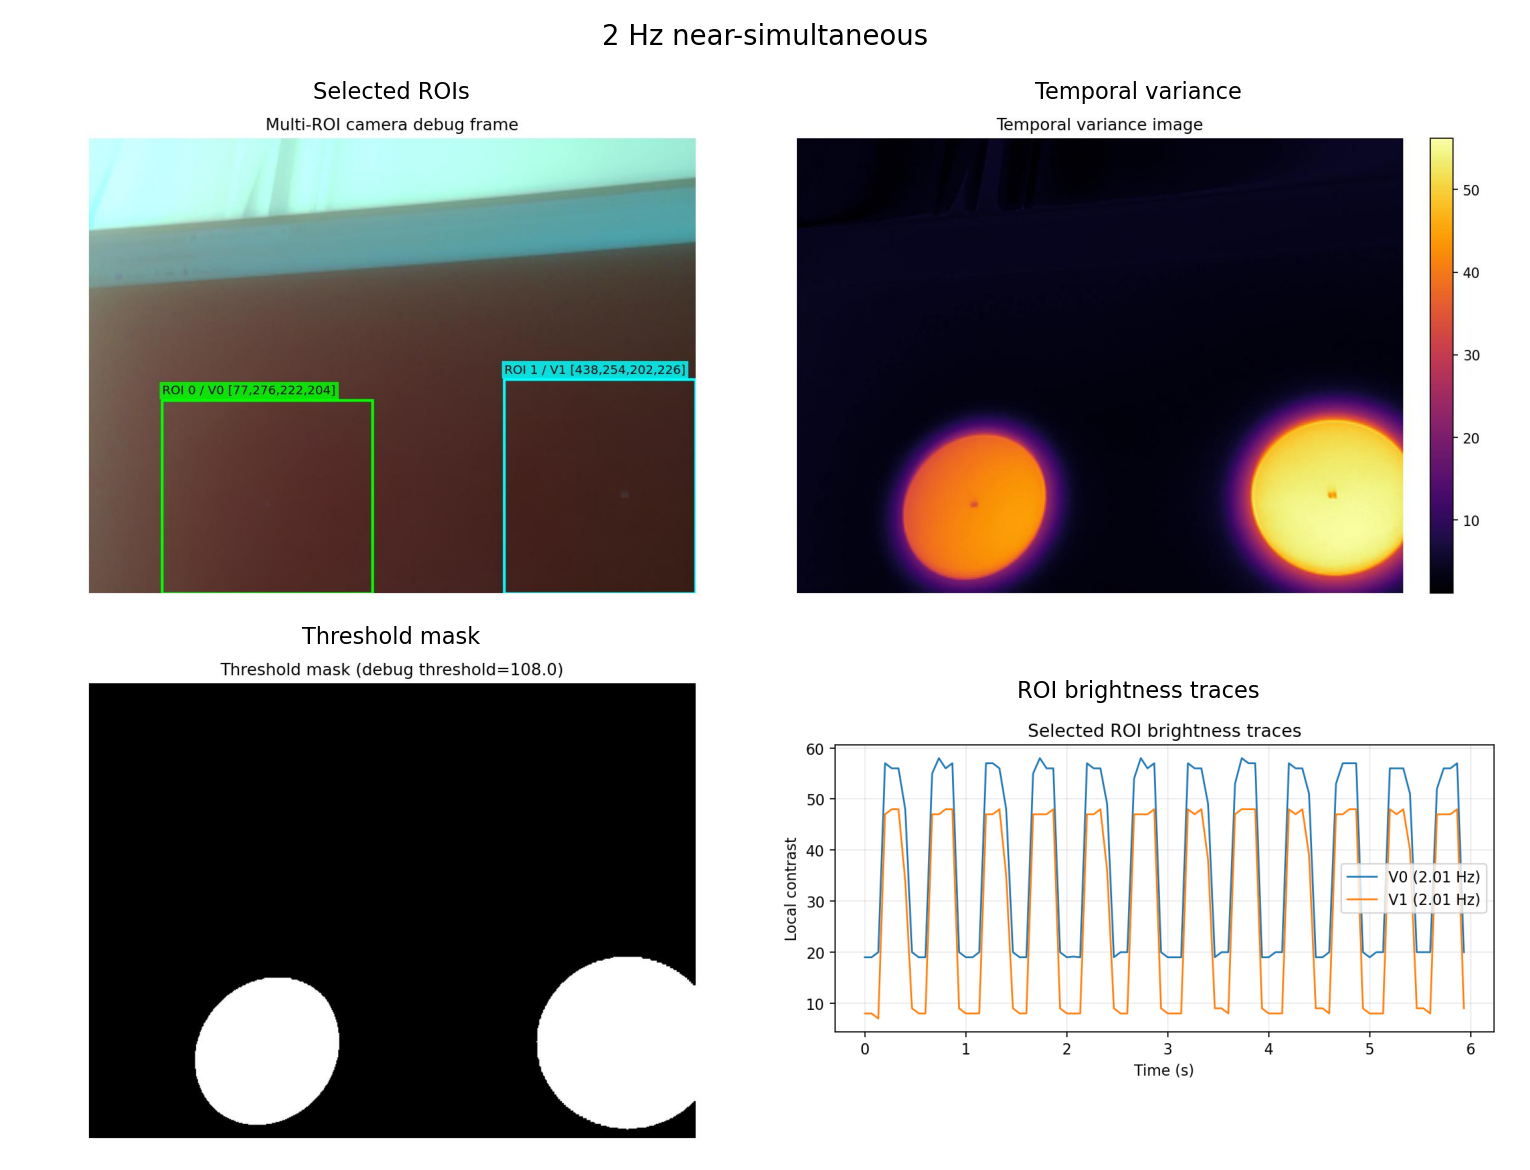
\includegraphics[width=0.95\textwidth]{figures/appendix/frequency_2hz_near_simultaneous_diagnostic_grid.png}
\caption{Auto-ROI diagnostics for 2 Hz near-simultaneous.}
\end{figure}

\begin{figure}[htbp]
\centering
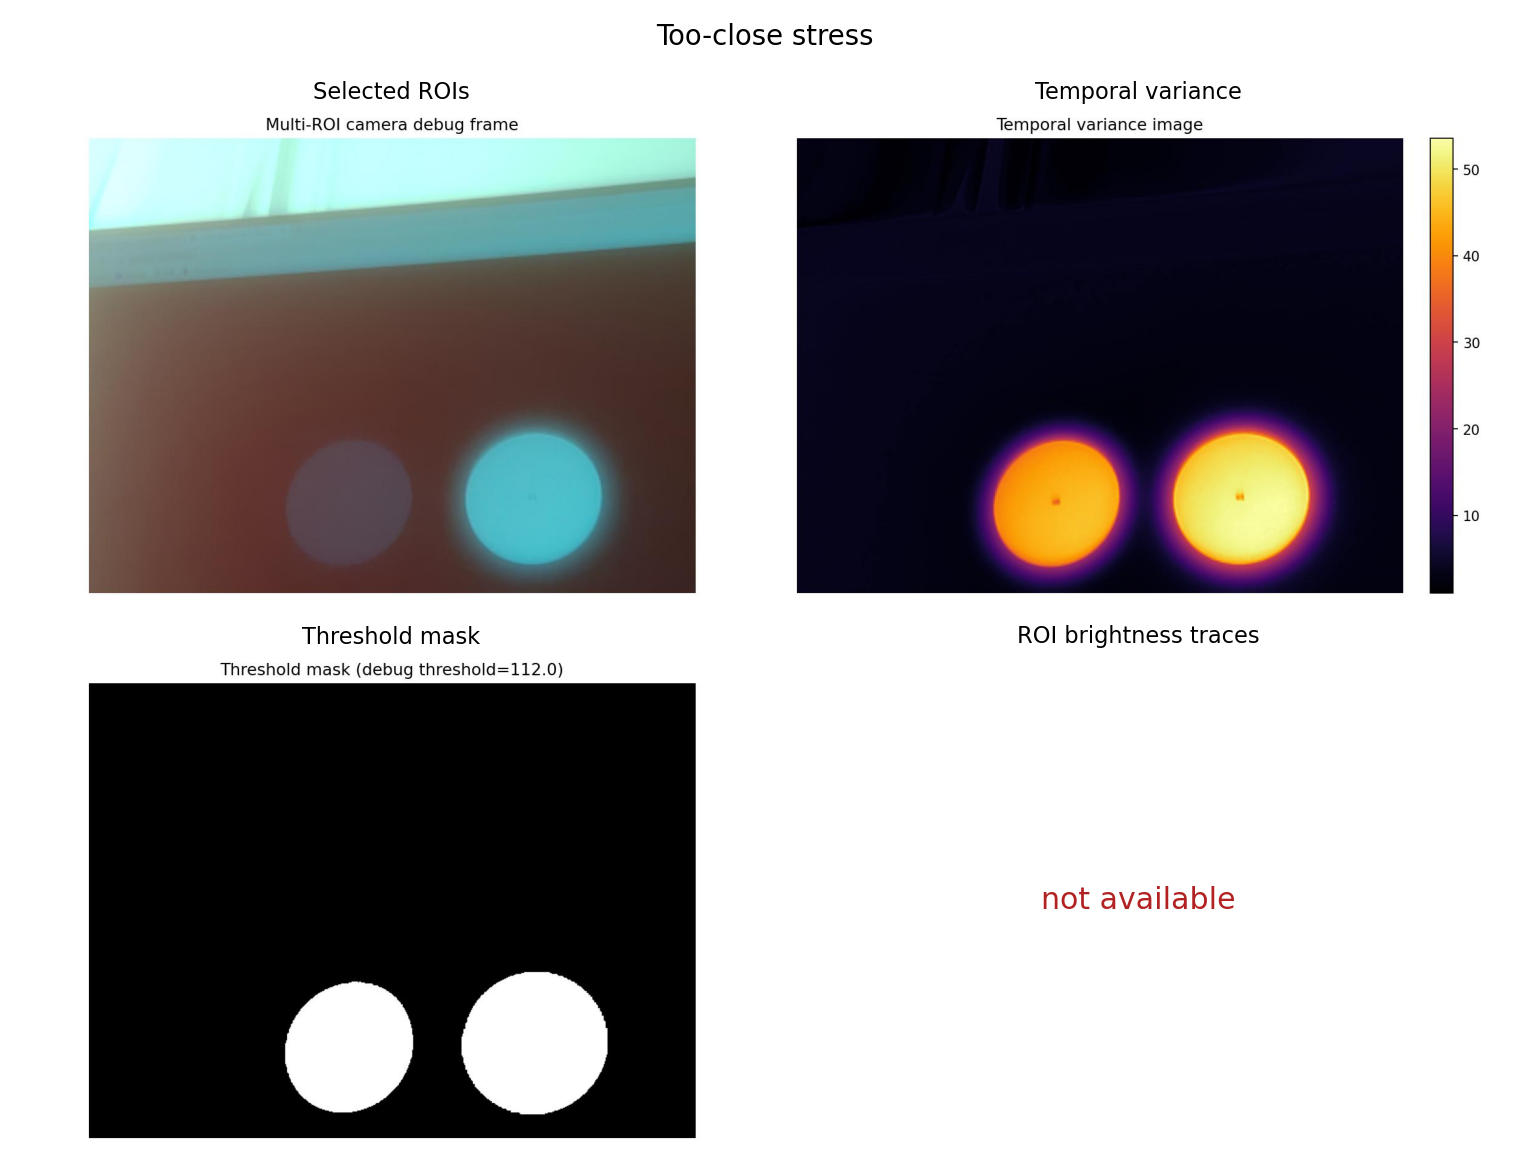
\includegraphics[width=0.95\textwidth]{figures/appendix/position_too_close_stress_diagnostic_grid.png}
\caption{Auto-ROI diagnostics for Too-close stress.}
\end{figure}

\begin{figure}[htbp]
\centering
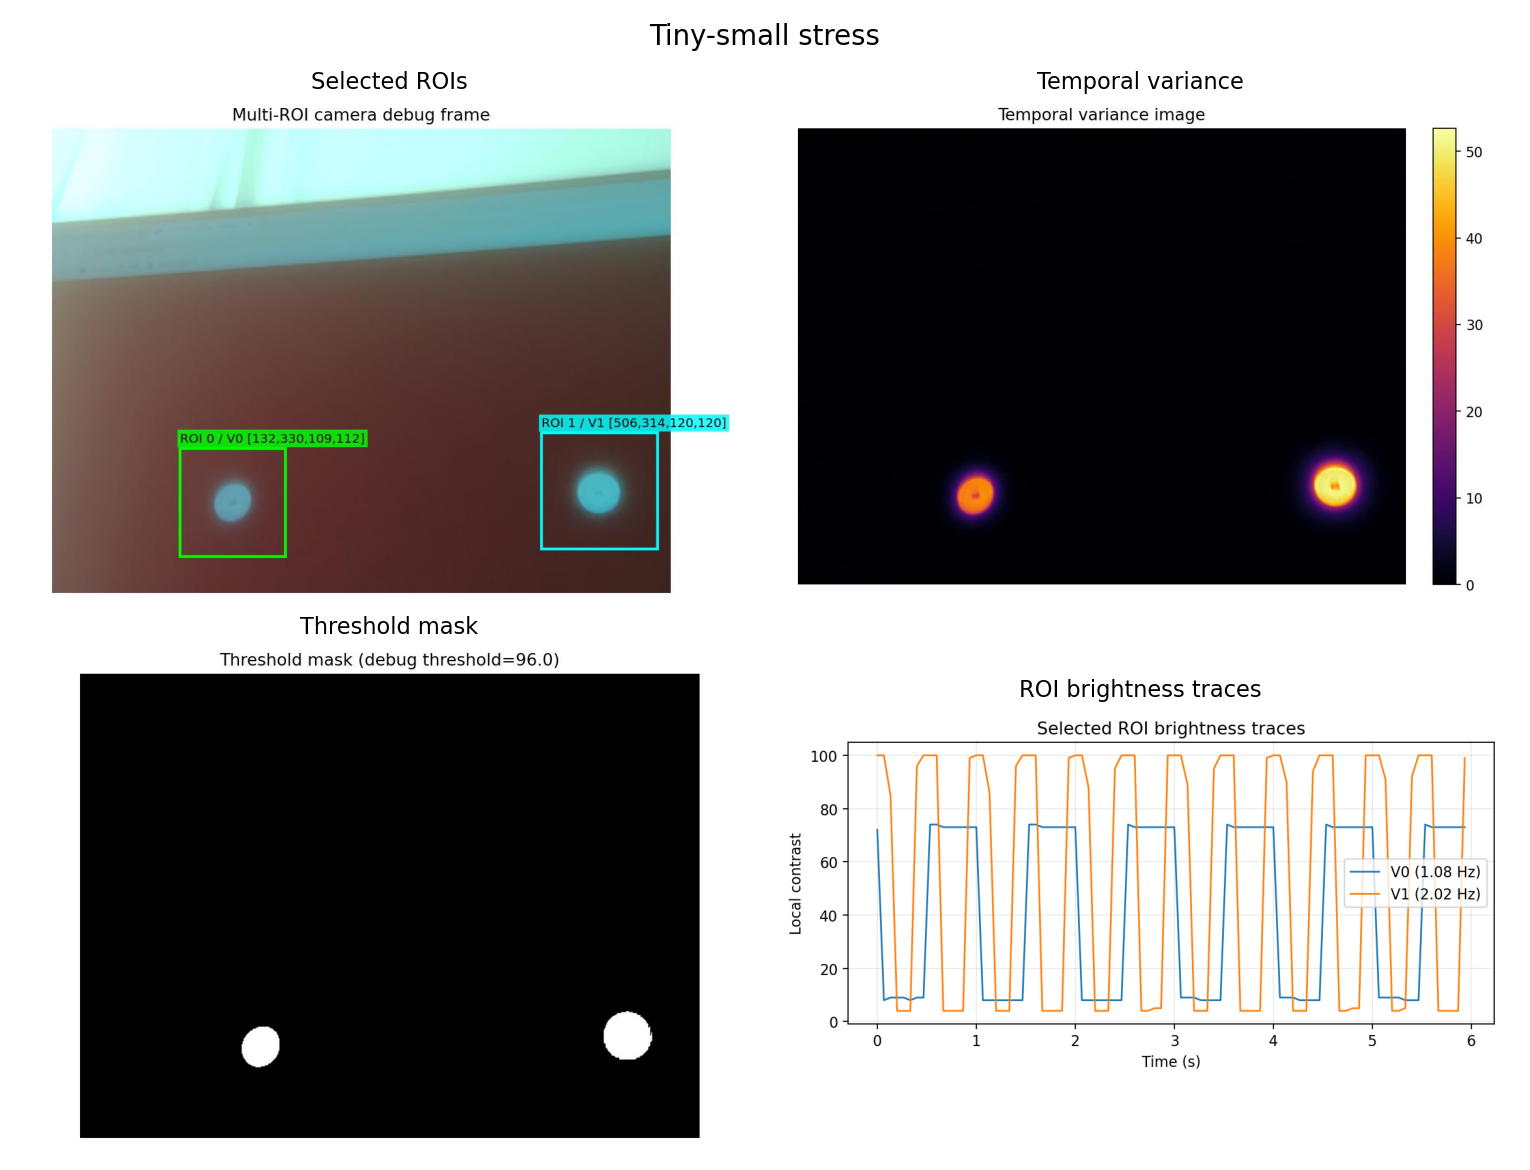
\includegraphics[width=0.95\textwidth]{figures/appendix/tiny_small_small_stress_diagnostic_grid.png}
\caption{Auto-ROI diagnostics for Tiny-small stress.}
\end{figure}

\begin{figure}[htbp]
\centering
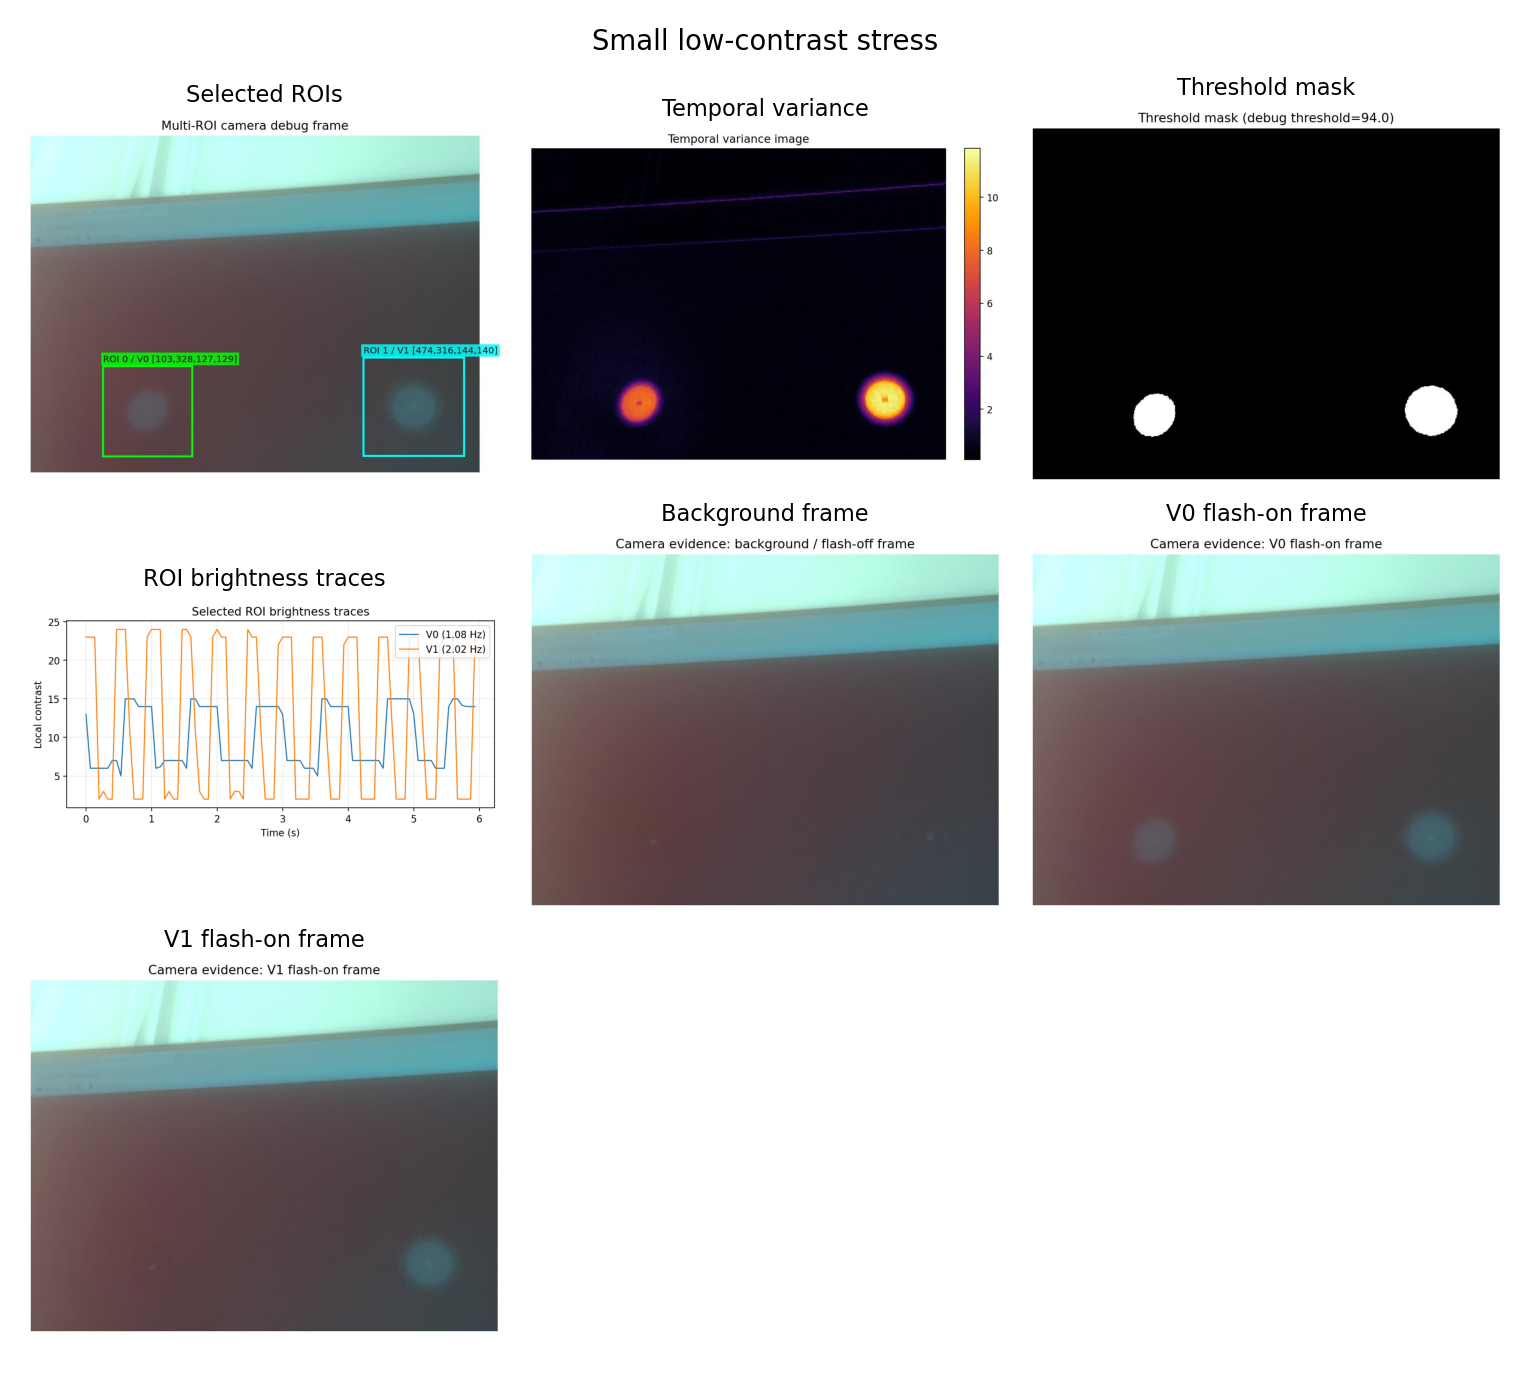
\includegraphics[width=0.95\textwidth]{figures/appendix/small_low_contrast_stress_diagnostic_grid.png}
\caption{Auto-ROI diagnostics for Small low-contrast stress.}
\end{figure}

\section{Reproducibility}

This report was generated by running
\path{python generate_step5c1_report.py} from
\path{docs/step5c1_multi_roi_detection_report/}. The LaTeX source is
\path{step5c1_multi_roi_detection_report.tex}. The PDF can be rebuilt with
\path{pdflatex step5c1_multi_roi_detection_report.tex}.

\end{document}
